\documentclass[11pt,a4paper]{article}
\usepackage{amsmath,amsthm,amssymb}
\RequirePackage{tikz}
\usetikzlibrary{calc,fit,arrows.meta}
\usepackage{pgfplots}
\pgfplotsset{compat=1.3}

\begin{document}

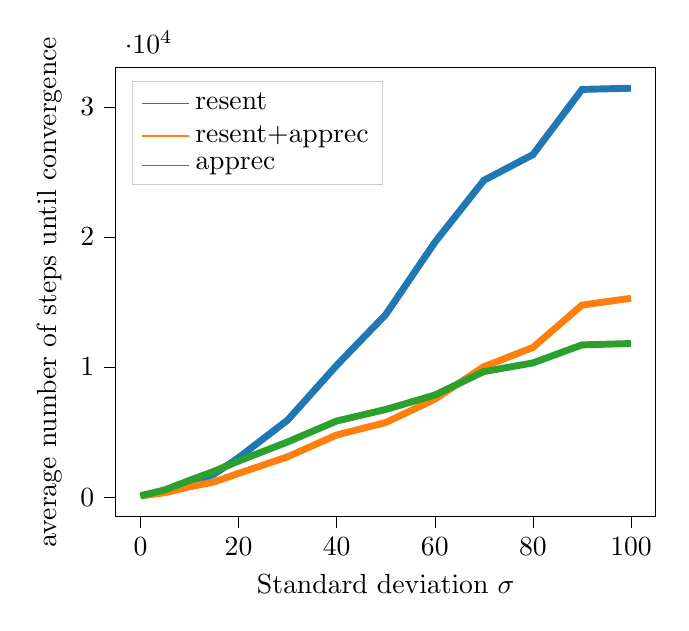
\begin{tikzpicture}[every plot/.append style={line width=2.5pt}]

\definecolor{color0}{rgb}{0.12156862745098,0.466666666666667,0.705882352941177}
\definecolor{color1}{rgb}{1,0.498039215686275,0.0549019607843137}
\definecolor{color2}{rgb}{0.172549019607843,0.627450980392157,0.172549019607843}

\begin{axis}[
legend cell align={left},
legend style={fill opacity=0.8, draw opacity=1, text opacity=1, at={(0.03,0.97)}, anchor=north west, draw=white!80!black},
tick align=outside,
tick pos=left,
x grid style={white!69.0196078431373!black},
xmin=-5, xmax=105,
xtick style={color=black},
y grid style={white!69.0196078431373!black},
ymin=-1466.9635, ymax=33008.2135,
ytick style={color=black},
ylabel={average number of steps until convergence},
xlabel={Standard deviation $\sigma$}
]
\addplot [semithick, color0]
table {%
0 102.22
5 389.8
10 1079.06
15 1757.62
20 3031.26
30 5920.41
40 10132.1313131313
50 14034.96
60 19584.1612903226
70 24355.7922077922
80 26335.0576923077
90 31348.1081081081
100 31441.16
};
\addlegendentry{resent}
\addplot [semithick, color1]
table {%
0 100.09
5 337.73
10 788.25
15 1161.13
20 1821.33
30 3098.81
40 4776.37
50 5730.03
60 7523.81
70 10029.04
80 11505.55
90 14762.68
100 15290.66
};
\addlegendentry{resent+apprec}
\addplot [semithick, color2]
table {%
0 101.61
5 559.99
10 1282.87
15 1985.18
20 2770.62
30 4241.53
40 5850.48
50 6736.6
60 7846.21
70 9652.96
80 10314.18
90 11704.36
100 11807.44
};
\addlegendentry{apprec}
\end{axis}

\end{tikzpicture}

\end{document}